% ============================================================================
%  TrustFin-SLM — Phase-4 Conference-Paper Draft
%  Execution-Verified Generation with Agreement-Calibrated Abstention
%  for Trustworthy Small Language Models in Finance
%
%  DRAFT (guide stage 15,17,19,20). Compiles with plain pdflatex (article class).
%  For submission, switch to the venue's class (IEEEtran / ACL acl-latex) —
%  content is 1:1, only the header changes. All claims sourced from
%  docs/exp_4(a).md, docs/exp_4(b).md and the phase-4 freeze manifests.
% ============================================================================
\documentclass[10pt]{article}
\usepackage[margin=1in]{geometry}
\usepackage[utf8]{inputenc}
\usepackage[T1]{fontenc}
\usepackage{lmodern}
\usepackage{microtype}
\usepackage{amsmath,amssymb}
\usepackage{booktabs}
\usepackage{graphicx}
\usepackage[table]{xcolor}
\usepackage{enumitem}
\usepackage{algorithm}
\usepackage{algpseudocode}
\usepackage{url}
\usepackage[round]{natbib}
\usepackage[colorlinks=true,linkcolor=blue,urlcolor=blue,citecolor=blue]{hyperref}
\usepackage{caption}
\captionsetup{font=small,labelfont=bf}

\newcommand{\ourmethod}{EVG-CAS}
\newcommand{\RR}{\mathcal{R}}
\newcommand{\CC}{\mathcal{C}}
\newcommand{\p}{\hat p}
\title{\textbf{Execution-Verified Generation with Agreement-Calibrated Abstention for Trustworthy Small Language Models in Finance}}
\author{Heet Mehta, Krish Patel, and Aryan Patel\\\small \href{mailto:heetmehta.work@gmail.com}{heetmehta.work@gmail.com} $\cdot$ \href{mailto:krishpatel19.tech@gmail.com}{krishpatel19.tech@gmail.com} $\cdot$ \href{mailto:aryanpatel26.ce@gmail.com}{aryanpatel26.ce@gmail.com}\\[2pt]\small {\em TrustFin-SLM Research Project}}
\date{\today}

\begin{document}
\maketitle

\begin{abstract}
Programmatic numerical reasoning benchmarks such as FinQA let a language model compute an
answer by \emph{executing the program it writes} against the official evaluator. We add
\ourmethod{} to a frozen, QLoRA-adapted 1.7B financial model, with one study question:
does paying a $3.7\times$ sampling cost for execution-verified generation make the model
\emph{more accurate}, \emph{more calibrated}, or both? Pre-registered on validation data
before the protected test was opened, the answer is threefold and honest. (1) It does
\textbf{not} make the model more accurate: on the protected FinQA held-out test,
execution-verified selection (65.56\%) statistically ties the frozen greedy baseline
(65.74\%), a negative result we report rather than bury. (2) It transforms
\emph{trustworthiness}: the agreement among the model's own executed answers is a steep,
monotone correctness signal (2.9\% $\rightarrow$ 79.2\% accuracy across agreement bins)
that is nearly invisible to the model's own log-probabilities (ROC-AUC 0.58). (3) Calibrating
that signal with out-of-fold Platt scaling produces a pre-registered abstention rule that
\emph{transfers}: at an 80\% coverage target frozen on validation, the protected test
suffers 31.0\% fewer errors among the answers it keeps (76.25\% accuracy), vs.\ 34.2\%
predicted. On FiQA the abstention benefit is negligible, and we report that too. A zero-shot
probe on FinBen-FOMC shows the frozen adapter also improves out-of-domain stance
classification (macro-F1 0.21 $\rightarrow$ 0.30, parse 0.90 $\rightarrow$ 0.99).
Generation-level verification does not make a benchmark-tuned small model \emph{right}
more often; it makes it \emph{know when it is wrong}, which is the property finance
deployment actually needs.
\end{abstract}

\noindent\textbf{Keywords:} small language models, financial reasoning, selective prediction,
calibration, execution-verified generation, abstention, FinQA, FiQA, FOMC.

\section{Introduction}\label{sec:intro}
Autoregressive language models are now small enough to run on a laptop and strong enough to
reason over financial documents \citep{phogat2024finetuning,chen2021finqa}. The remaining
obstacle to deploying a 1.7B model in finance is not raw accuracy, it is \emph{trust}: a
financial system that silently gives a wrong number to a user is unusable even if it is
right 65\% of the time. Benchmarks have begun to measure this deficit --- FinTrust lists
``appropriately abstain when confidence is low'' as a first-class trustfulness dimension
\citep{hu2025fintrust} --- but they diagnose it on GPT-4-scale models and provide no
mechanism a small model can actually use.

This paper provides the mechanism, and reports the outcome honestly. We study a task class
where \emph{execution} is a well-defined ground-truth operation: programmatic numerical
reasoning \citep{chen2021finqa}. The model writes a program; the answer is what the
program computes. That property lets us sample $n$ candidate programs per question, keep
only those that run on the official evaluator, and observe how much the surviving \emph{answers}
agree. Prior work uses such sampling to \emph{vote} (self-consistency \citep{wang2023selfconsistency})
or to train outcome/process reward models \citep{lightman2024verify,wang2024mathshepherd},
framing the payoff as accuracy. We find, on protected data, that framing is wrong for our
model: execution-verified selection does not beat the greedy baseline (Table~\ref{tab:c1}).
We therefore spend the sampling budget where it pays: agreement is a trust feature, and a
calibrated, pre-registered abstention policy built on it cuts protected-test answered-error
by 31\% at 80\% coverage (Table~\ref{tab:transfer}).

Our contributions. \textbf{(C1)} An honest, pre-registered accuracy verdict: EVG does not
improve FinQA/FiQA accuracy for a QLoRA-tuned 1.7B model; it ties it. \textbf{(C2)} A
calibration construction that gives the model probability-meaningful confidence, cutting
Brier 0.28$\rightarrow$0.16 and ECE 0.26$\rightarrow$0.05. \textbf{(C3)} A selective-prediction
policy whose threshold is fixed on validation and whose benefit transfers to a protected
test ($-$31.0\% test answered-error reduction at coverage 0.8, predicted $-$34.2\%).

\section{Related work}
\paragraph{Small financial models and adaptation.}
Survey evidence shows 1--3B models are a deliberate performance/efficiency point
\citep{subramanian2025slms,abdin2024phi3,zhang2024tinyllama}, and LoRA/QLoRA make domain
adaptation cheap \citep{hu2022lora,dettmers2023qlora}. Financial-domain adaptation builds
on this for QA and sentiment \citep{phogat2024finetuning,yang2023fingpt,yang2023investlm,wu2023bloomberg,huang2020finbert,shi2025kronos}.
The closest comparable work, fine-tuning smaller models on FinQA \citep{phogat2024finetuning},
also operates in our compute regime and reports accuracy only --- as we do, but we add the
trust layer it omits.

\paragraph{Programmatic financial reasoning.}
FinQA \citep{chen2021finqa}, ConvFinQA \citep{chen2022convfinqa} and TAT-QA
\citep{zhu2021tatqa} establish that execution (running the program) is the ground truth of
the answer. FinBen \citep{xie2024finben} supplies the benchmarking context including the
FiQA and FOMC tasks we use; FinTrust \citep{hu2025fintrust} establishes abstention as a
measured trust deficit.

\paragraph{Consistency and verification.}
Self-consistency votes over sampled paths \citep{wang2023selfconsistency}; process-supervised
verifiers rerank candidates with a learned model \citep{lightman2024verify,wang2024mathshepherd};
execution-guided synthesis filters decoding by the runtime \citep{chen2019execution}.
All are accuracy-centric. Ours re-purposes their machinery as a \emph{decision signal}.

\paragraph{Selective prediction and calibration.}
The risk-coverage framework \citep{eliyaniv2010selective,geifman2017selective,geifman2019selectivenet}
defines abstention evaluation; Platt/isotonic/temperature calibration
\citep{platt1999platt,zadrozny2002isotonic,guo2017calibration} and verbalised uncertainty
\citep{lin2022uncertainty} provide LLM confidence. Responsible-AI guidance in finance
\citep{fritzmorgenthal2022risk} is the regulatory motivation.

\section{Problem statement and protocol}
\paragraph{Setup.} A question $q$ maps to a program $p$; the answer is $a=\text{exec}(p)$
if $p$ is valid. The model is a frozen, domain-adapted SLM $\pi_{\theta}$. We pre-declare
three claims (fixated in \texttt{PLAN.md} before any protected-test access):
\begin{itemize}[nosep,leftmargin=1.2em]
\item \textbf{C1 (accuracy):} execution-verified selection improves the answer's
execution-ground-truth accuracy over greedy decoding.
\item \textbf{C2 (probability quality):} calibrating trust features lowers Brier score and
ECE and makes a coverage threshold carry probability meaning.
\item \textbf{C3 (ranking):} trust features from the sample population (agreement,
executability) improve the calibrator's ordering, measurable as a drop in expected AURC,
whenever the features are non-monotone with the raw confidence.
\end{itemize}
\paragraph{Guardrails (integrity before novelty).} All selection of the model, the method
and the hyper-parameters ($n=8$, temperature 0.7, top-$p$ 0.9, 5-fold out-of-fold
calibration, coverage targets \{0.80, 0.90\}) happened on \emph{validation} data only. The
protected test sets were opened exactly once, after a freeze manifest registered status
\texttt{FROZEN} and the run set an explicit protected flag; a SHA-256 of the freeze was
recorded before and after the test run and is unchanged. The full integrity protocol is
documented in \$6 of \texttt{docs/exp\_4(a).md}.

\section{Method: \ourmethod{}}\label{sec:method}

\subsection{Sampling and execution verification}
Given $q$, sample $n$ programs $p^{(1)},\dots,p^{(n)}\sim\pi_{\theta}(\cdot\mid q)$
(temperature 0.7, top-$p$ 0.9, no other search). Each $p^{(i)}$ is run with the official
evaluator if it parses; an answer $a^{(i)}$ exists iff the program is valid and executes.
Evidence is carried by the \emph{candidate population}, not by any single decode.

\subsection{Trust features from the sample population}
For a question $q$ with $n$ candidates we compute three pre-registered features:
\begin{align}
  \text{agreement} \quad &\mathcal{A}(q) \;=\; \frac{1}{n(n-1)}\sum_{i\neq j}
    \mathbb{1}[a^{(i)} = a^{(j)}],\\
  \text{executability} \quad &\mathcal{R}(q) \;=\; \frac{1}{n}\sum_{i=1}^{n}
    e^{(i)}, \qquad e^{(i)} = \mathbb{1}[\,p^{(i)}\ \text{valid}\ \wedge\ a^{(i)}\ \text{exists}\,],\\
  \text{self-confidence} \quad &\mathcal{C}(q) \;=\; \overline{\log\pi_{\theta}(p^{(\star)}\mid q)},
\end{align}
where $p^{(\star)}$ is the selected candidate and the mean is over its tokens.
The feature vector is $f(q)=[\mathcal{A}(q),\,\mathcal{R}(q),\,\mathcal{C}(q)]$. The gold
answer is used only to \emph{score} these features, never to select a candidate or a
threshold (guardrail: nothing refit on test).

\subsection{Calibration (C2)}
The score $\p(q) = \Pr[\text{answer is correct} \mid f(q)]$ is learned by out-of-fold
Platt scaling:
\begin{equation}
  \p(q) \;=\; \sigma\!\big(w\cdot f(q) + b\big), \qquad
  \sigma(z) = \frac{1}{1+e^{-z}} ,
\end{equation}
with $(w,b)$ fit by logistic regression on inner-fold predictions and applied to outer folds
(5 folds), so every validation prediction is genuinely out-of-sample. Because a single-feature
monotone calibrator cannot reorder answers, we evaluate \textbf{(i)} a single-feature baseline
($f=[\mathcal{C}]$) and \textbf{(ii)} the full feature vector $f$ \textbf{(C3)}.

\subsection{Freeze and abstention rule (C2)}
For coverage target $1-\alpha$ (pre-registered $\alpha \in \{0.20, 0.10\}$):
\begin{equation}
  \theta \;=\; \min\Big\{ t : \CC_{\text{val}}(t) \ge 1-\alpha \Big\},
  \qquad \CC(t) = \frac{1}{|V|}\sum_{q\in V}\mathbb{1}[\p(q)\ge t],
\end{equation}
and the decision rule on any future question is answer $q$ iff $\p(q) \ge \theta$, else abstain.
Selective risk and coverage follow \citep{eliyaniv2010selective}:
\begin{equation}
  \RR(\theta)=\frac{\sum_{q} \ell(q)\,\mathbb{1}[\p(q)\ge\theta]}
                   {\sum_{q}\mathbb{1}[\p(q)\ge\theta]}, \qquad
  \ell(q) = \mathbb{1}[\text{answer}(q)\neq \text{gold}(q)].
\end{equation}

\begin{algorithm}[t]
\caption{\ourmethod{} decision pipeline (fit once on validation; frozen thereafter)}
\begin{algorithmic}[1]
\Require frozen adapter $\pi_\theta$, sampler params $(n,\tau,p)$, evaluator $\text{exec}$, coverage targets
\State \textbf{Validation phase:}
\For{$q \in V$}
  \State sample $n$ programs; keep valid ones; get answers $a^{(i)}$
  \State compute $f(q)=[\mathcal{A}(q),\,\mathcal{R}(q),\,\mathcal{C}(q)]$
\EndFor
\State fit out-of-fold Platt $w,b$ on $(f(q),\,\ell(q))_{q\in V}$; score $\p(q)$ OOF
\State pick $\theta$ s.t.\ $\CC_{\text{val}}(\theta) \ge 1-\alpha$ for each target
\State write \texttt{phase4\_freeze.json} (FROZEN, $w,b,\theta,\alpha$, sha256)
\State \textbf{Protected phase (opened once, after FROZEN + protected flag):}
\For{$q \in T$}
  \State draw $n$ candidates; if $\p(q) \ge \theta$ emit answer$(q)$, else \textbf{abstain}
\EndFor
\end{algorithmic}
\end{algorithm}

\section{Experimental setup}\label{sec:setup}
\paragraph{Data and aligned evaluation.}
FinQA (train 6\,251 / validation 883 / held-out test 1\,147) uses the official program
evaluator; we report three aligned accuracies: \emph{printed} (the answer string the model
emits), \emph{program} (does the parse succeed), and \emph{execution} (does the executed
answer match gold). FiQA (validation 117 / test 234) is regression with MAE, $R^2$,
Pearson $r$ at tolerance 0.10. FOMC (test 496: neutral 245, dovish 129, hawkish 122) is
zero-shot stance classification with accuracy, macro-F1 and parse success.
\paragraph{Model.} Frozen Phase-3 winner: \texttt{Qwen/Qwen3-1.7B}
\citep{qwen2025qwen3} with balanced-joint QLoRA \citep{dettmers2023qlora} as canonical on
FinQA and explicit-schema on FiQA; exact hyper-parameters are in
\texttt{phase3\_freeze.json} and were fixed before this work began.
\paragraph{Metrics.} Brier, ECE-10, expected AURC (e-AURC; lower is better), coverage and
selective risk. All numbers cited as ``validation'' are out-of-fold or tuned on
validation; all ``test'' numbers were produced by the frozen system and are unchanged since
the completed protected run \citep{see exp\_4(b).md}.

\begin{table}[t]
\centering
\caption{\label{tab:c1} C1 evidence. \textbf{(top)} FinQA held-out test, execution accuracy
per rule ($n{=}8$); \textbf{(bottom)} FiQA test regression. EVG neither beats nor loses to
the frozen greedy baseline on either task; per-record, 18 questions are won and 20 lost.}
\small
\begin{tabular}{lc}
\toprule
\multicolumn{2}{l}{\emph{FinQA test, execution accuracy ($n{=}1147$)}}\\
\midrule
frozen greedy (baseline) & \textbf{0.6574}\\
candidate-0 (prints) & 0.6399\\
self-consistency vote & 0.6478\\
best-of-$n$ & 0.6556\\
\textbf{execution-verified (ours)} & 0.6556\\
\bottomrule
\end{tabular}
\vspace{0.5em}
\begin{tabular}{lcc}
\toprule
\multicolumn{3}{l}{\emph{FiQA test ($n{=}234$), MAE / accuracy@0.10}}\\
\midrule
frozen greedy & \textbf{0.1301} & \textbf{0.568}\\
median-of-$n$ (ours) & 0.1306 & 0.556\\
\bottomrule
\end{tabular}
\end{table}

\begin{table}[t]
\centering
\caption{\label{tab:agreement} Agreement bins vs.\ correctness on the protected test.
Agreement is steeply and monotonically predictive: the model knows its own confidence
regime even though its log-probability cannot separate correct from incorrect answers
(ROC-AUC 0.58).}
\small
\begin{tabular}{lcc}
\toprule
EVG agreement bin & $n$ records & execution accuracy\\
\midrule
(0.00, 0.25] & 35 & \textbf{0.029}\\
(0.25, 0.50] & 122 & 0.238\\
(0.50, 0.75] & 181 & 0.448\\
(0.75, 1.00] & 809 & \textbf{0.792}\\
\bottomrule
\end{tabular}
\end{table}

\begin{table}[t]
\centering
\caption{\label{tab:calib} C2/C3 calibration results on FinQA validation (out-of-fold).
\emph{Top:} ordering quality (e-AURC, lower better). Single-feature calibrators do not move
the raw ranking (a monotone map cannot); the agreement-driven full vector does ($-$39.3\%).
\emph{Bottom:} probability quality of the frozen policy.}
\small
\begin{tabular}{lcc}
\toprule
\multicolumn{3}{l}{\emph{e-AURC on FinQA validation (frame = exec-verified)}}\\
\midrule
raw confidence & 0.2029\\
+ isotonic (feature: confidence) & 0.2028\\
+ Platt (feature: confidence) & 0.2496\\
\rowcolor{gray!15} \textbf{+ Platt (features: agree, exec, conf)} & \textbf{0.1232}\\
\multicolumn{3}{l}{\quad baseline greedy frame, best method: 0.1897}\\
\midrule
\multicolumn{3}{l}{\emph{Probability quality (frozen FinQA policy)}}\\
\midrule
raw confidence / Platt full & Brier 0.2845~$\rightarrow$~\textbf{0.1579} & ECE 0.2555~$\rightarrow$~\textbf{0.0475}\\
\bottomrule
\end{tabular}
\end{table}

\begin{table}[t]
\centering
\caption{\label{tab:transfer} Transferred abstention (frozen thresholds, protected test).
The threshold and calibration were fixed on validation \emph{before} the test opened; the
realised behaviour is close to predicted ($-$31.0\% vs\ $-$34.2\%). FiQA, as pre-frozen on
raw confidence, abstains to no effect ($-$2.9\%).}
\small
\begin{tabular}{lcccccc}
\toprule
\multicolumn{7}{l}{\emph{FinQA (frozen: exec-verified + Platt-full + $\theta$)}}\\
\toprule
target & $\theta$ & test cov. & select. risk & selected acc. & abstained & err.\ rel.\ $\Delta$\\
\midrule
0.80 & 0.409 & 0.786 & \textbf{0.2375} & \textbf{0.7625} & 246 & \textbf{$-$31.0\%}\\
0.90 & 0.221 & 0.926 & 0.3004 & 0.6996 & 85 & $-$12.8\%\\
\bottomrule
\end{tabular}
\vspace{0.4em}
\begin{tabular}{lcccc}
\toprule
\multicolumn{5}{l}{\emph{FiQA (frozen: greedy + raw confidence)}}\\
\toprule
target & test cov. & select. risk & full risk & err.\ rel.\ $\Delta$\\
\midrule
0.80 & 0.765 & 0.4190 & 0.4316 & $-$2.9\%\\
0.90 & 0.885 & 0.4203 & 0.4316 & $-$2.6\%\\
\bottomrule
\end{tabular}
\end{table}

\begin{table}[t]
\centering
\caption{\label{tab:rigor} Evaluation rigor on the protected test (n=1,147). \textbf{(top)}
Paired comparison: the C1 tie is statistically verified, not read off rounded means.
\textbf{(middle)} Error taxonomy: the only channel EVG fails to fix is the \emph{printed}
answer string. \textbf{(bottom)} Reasoning-depth stratification: abstention concentrates on
the deepest programs and delivers its largest relative gain there. Bootstrap CI: 10{,}000
resamples; McNemar exact (binomial).}
\small
\begin{tabular}{lcc}
\toprule
\multicolumn{3}{l}{\emph{C1 significance (protected test, paired)}}\\
\toprule
 & greedy & exec-verified\\
\midrule
execution acc. & 0.6574 & 0.6556\\
delta & \multicolumn{2}{c}{$-0.0017$ \quad 95\% CI $[-0.0122,\,+0.0087]$}\\
McNemar exact $p$ & \multicolumn{2}{c}{0.871}\\
\bottomrule
\end{tabular}
\vspace{0.6em}
\begin{tabular}{lr}
\toprule
\multicolumn{2}{l}{\emph{Error taxonomy of wrong answers}}\\
\midrule
& \emph{n} (\%) \\
parse failure & 0 (0.0)\\
invalid/unexecutable program & 0 (0.0)\\
executes but wrong & 395 (34.4)\\
executes right, prints wrong string & 0 (0.0) \\
\emph{greedy} executes right, prints wrong string & 355 (31.0)\\
\bottomrule
\end{tabular}
\vspace{0.6em}
\begin{tabular}{lrrrr}
\toprule
program ops & $n$ & full acc. & selected acc. & err.\ $\Delta$\\
\midrule
0 & 45 & 0.844 & 0.884 & $-$25.2\%\\
1 & 644 & 0.649 & 0.764 & $-$32.6\%\\
2 & 391 & 0.662 & 0.748 & $-$25.2\%\\
3--6 & 67 & 0.552 & 0.739 & $-$41.7\%\\
\bottomrule
\end{tabular}
\end{table}

\begin{table}[t]
\centering
\caption{\label{tab:fomc} Zero-shot out-of-domain robustness on FinBen-FOMC (test, 496):
the frozen financial adapter improves the balanced metric and the rare classes that a
neutral-majority model otherwise ignores.}
\small
\begin{tabular}{lcccccc}
\toprule
system & accuracy & macro-F1 & parse & F1 dovish & F1 neutral & F1 hawkish\\
\midrule
base \texttt{Qwen/Qwen3-1.7B} & 0.454 & 0.215 & 0.899 & 0.163 & 0.650 & 0.046\\
\textbf{+ frozen E5 adapter} & 0.484 & \textbf{0.304} & \textbf{0.986} & 0.333 & 0.621 & 0.260\\
\bottomrule
\end{tabular}
\end{table}

\section{Results}\label{sec:results}
\paragraph{C1 is rejected --- and that is a result.}
Table~\ref{tab:c1}. On the protected test, execution-verified selection is 0.6556 vs.\
frozen greedy 0.6574 ($-$0.18~pp; per-record 18 gained, 20 lost, exact McNemar $p=0.871$,
bootstrap 95\% CI $[-0.0122,+0.0087]$), and the FiQA median-based
aggregator is 0.0005 worse in MAE. Validation showed the same story (tie: 0.6750 vs.\ 0.6750).
The one clean C1 win is \emph{program hygiene}: the invalid-program rate in the emitted
answers drops from $3.5\times10^{-3}$ to exactly \textbf{0}. Every answer we keep is backed
by a program the official evaluator accepted.

\paragraph{Agreement is the trust signal (C3 evidence at the decision level).}
Table~\ref{tab:agreement}. On protected data the
model reports perfect agreement on records that are 2.9\% correct and record-high agreement
on records that are 79.2\% correct; nothing in the model's own log-probability separates
these regimes (ROC-AUC 0.58). This is the signal that buys abstention.

\paragraph{Calibration gives the threshold meaning (C2).}
Table~\ref{tab:calib}. Out-of-fold Platt on the agreement features cuts Brier 0.28
$\rightarrow$ 0.16 and ECE 0.26 $\rightarrow$ 0.05. The ranking result is exactly what the
monotonicity caveat predicts: the single-feature calibrators cannot move e-AURC
(0.2029 $\rightarrow$ 0.2028), while the agreement-driven vector drops it to 0.1232
($-$39.3\% vs.\ raw, $-$35.1\% vs.\ the best baseline frame).

\paragraph{The frozen policy transfers (C2's operational payoff).}
Table~\ref{tab:transfer}. With the threshold fixed on validation, opening the protected test
once yields: coverage 0.786 at the 0.80 target, selective risk 0.2375 (accuracy 0.7625)
vs.\ 0.3444 at full coverage --- a \textbf{31.0\% relative error reduction}, against the
34.2\% predicted from validation; bootstrap 95\% CI on the reduction is $[22.8\%,\,39.3\%]$
(i.e.\ the transfer is significant, not a rounding effect). FiQA abstention is −2.9\%: as the frozen FiQA method (raw
confidence on greedy) predicted, its errors are not rankable.

\begin{figure}[t]
\centering
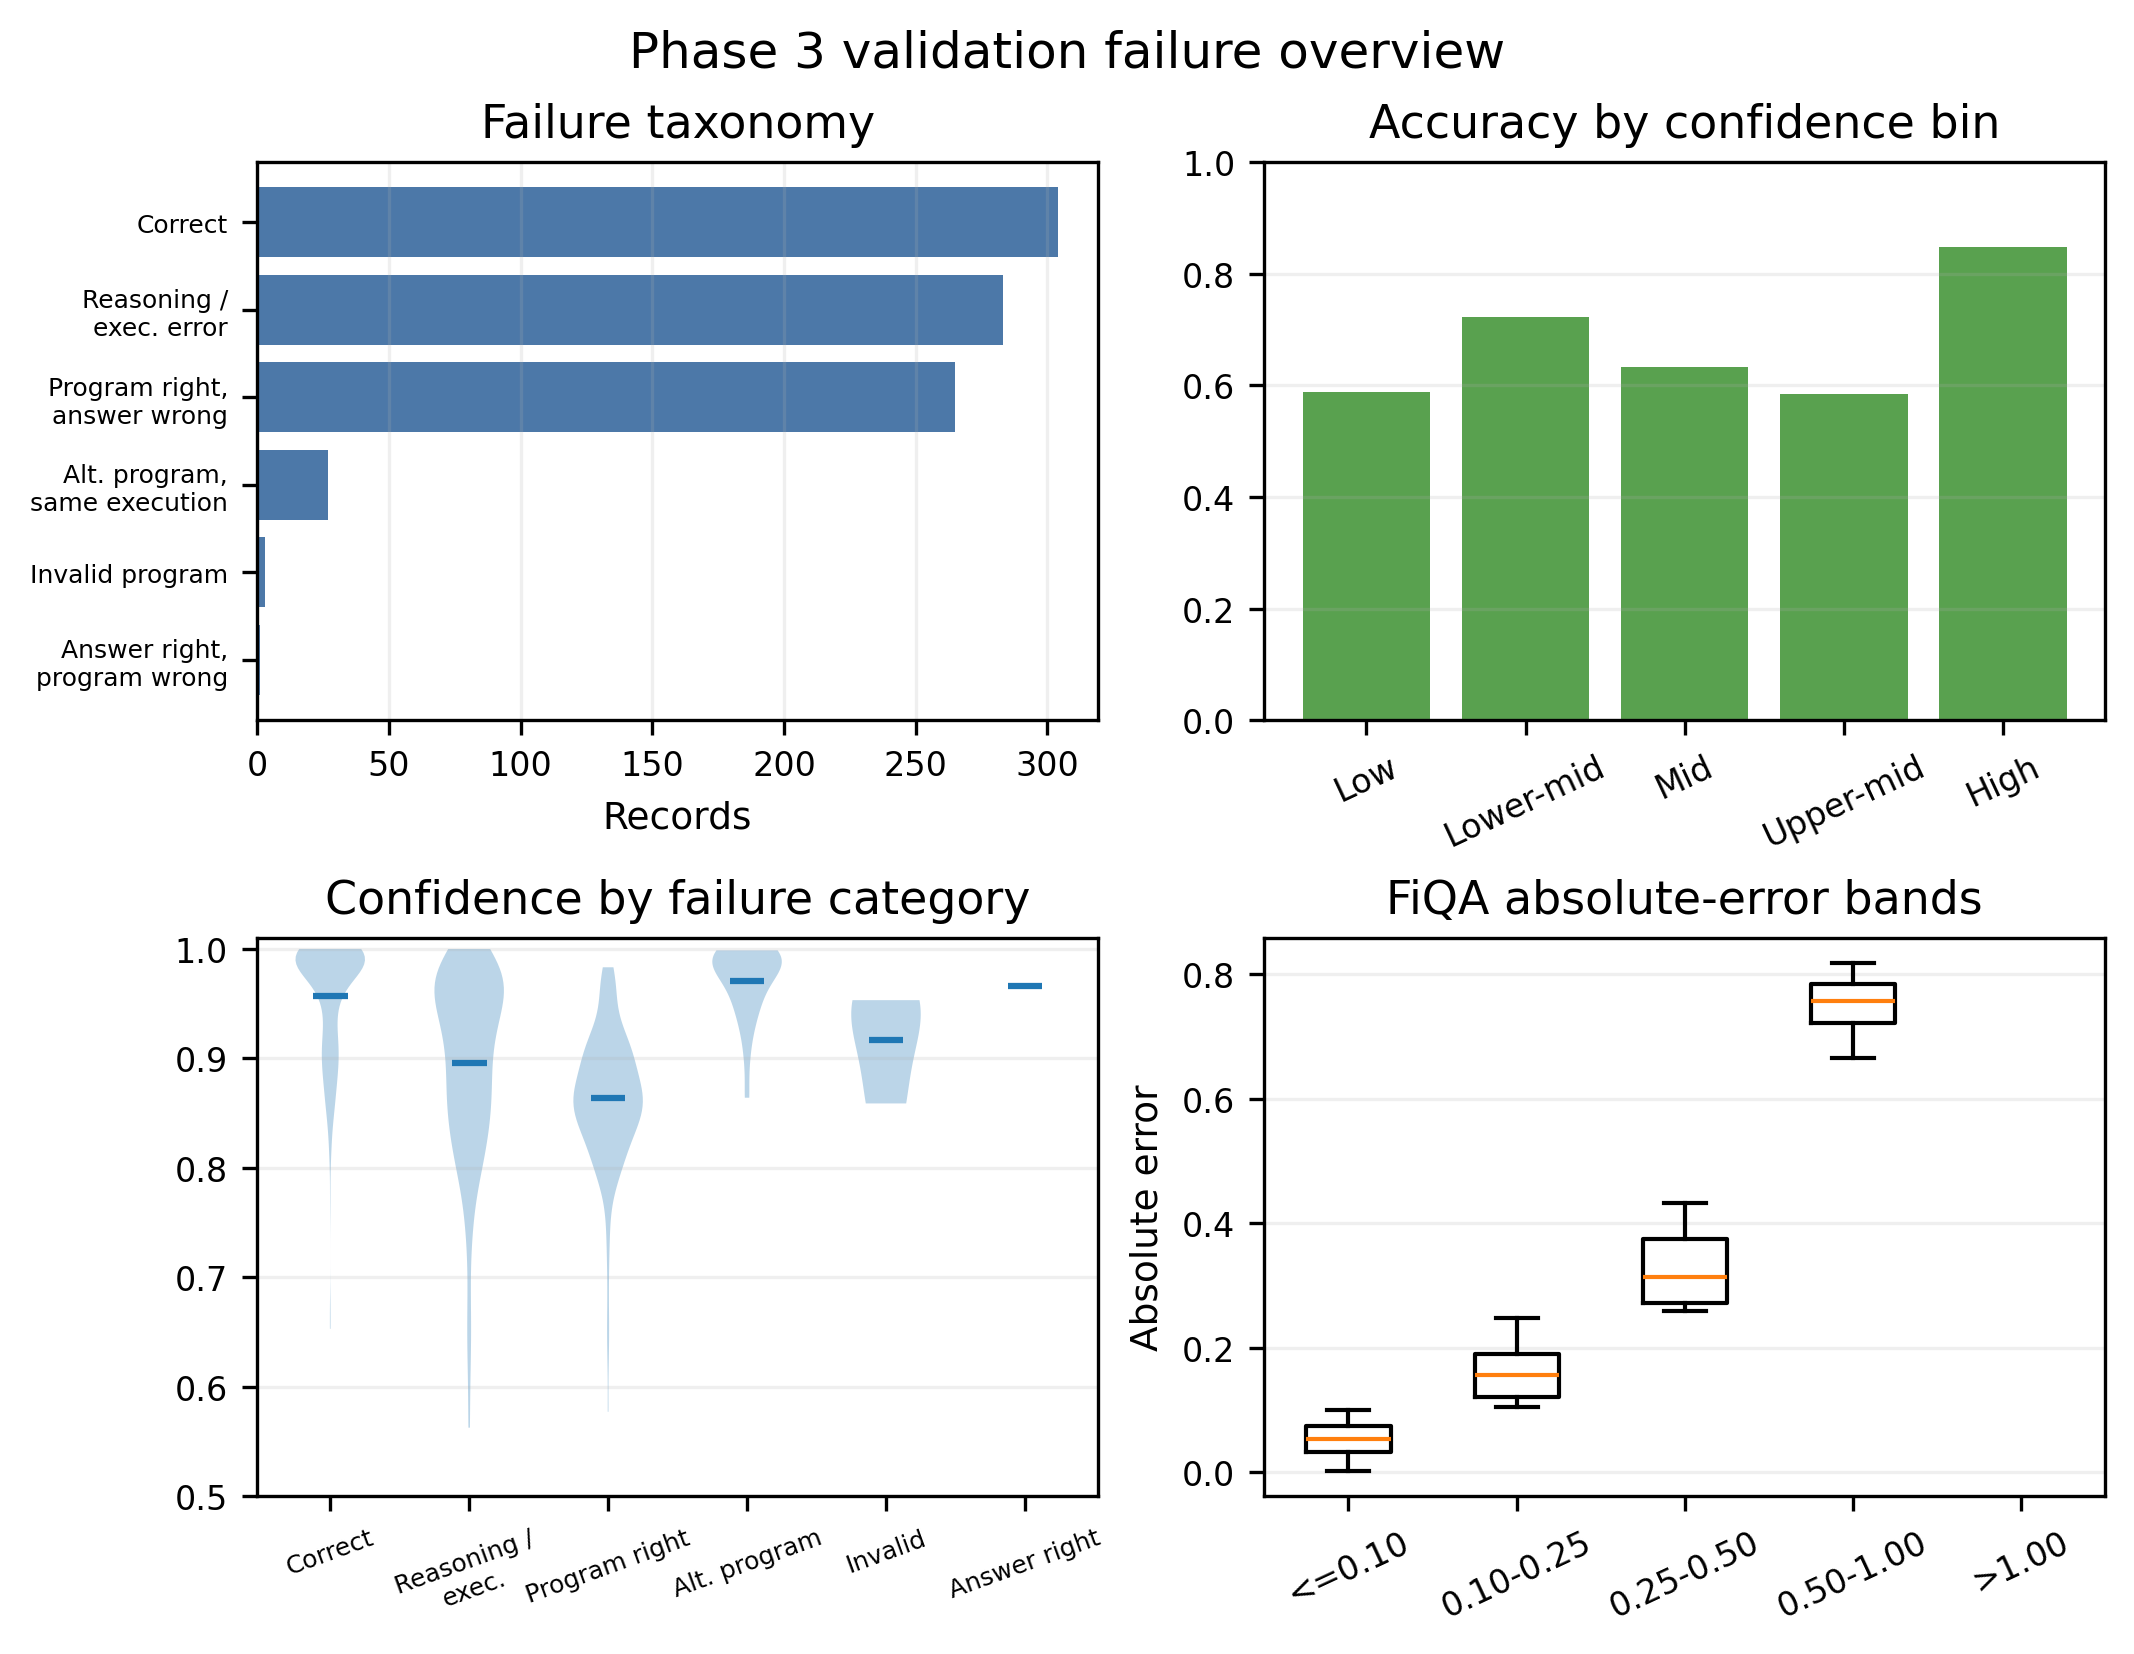
\includegraphics[width=\textwidth]{figures/fig6_finqa_failure_overview.png}
\caption{\label{fig:finqa_failure} FinQA failure distribution of the frozen E5 model on
validation ($n{=}883$). \textbf{(a)} Of all records, 34.4\% are correct; the residual is
dominated by two comparable channels --- reasoning/execution errors (32.0\%) where the
program is structurally valid but mis-specified, and program-right/answer-wrong cases
(30.0\%) that are mostly precision/rounding near-misses. \textbf{(b)} Self-reported
confidence barely separates correct from failed records (median $\approx$96\% in both the
correct and reasoning-error classes), consistent with the ROC-AUC 0.58 reported in
Table~\ref{tab:agreement}. \textbf{(c)} Accuracy does rise in the top confidence bins
(80.4\% in 99--100\%), but the mid-range is badly miscalibrated. \textbf{(d)} Failure
magnitude is bimodal: program-right/answer-wrong errors are near-misses (median relative
error 1.7\%), while reasoning/execution errors are catastrophic misreads (median
$\approx$99\%).}
\end{figure}

\begin{figure}[t]
\centering
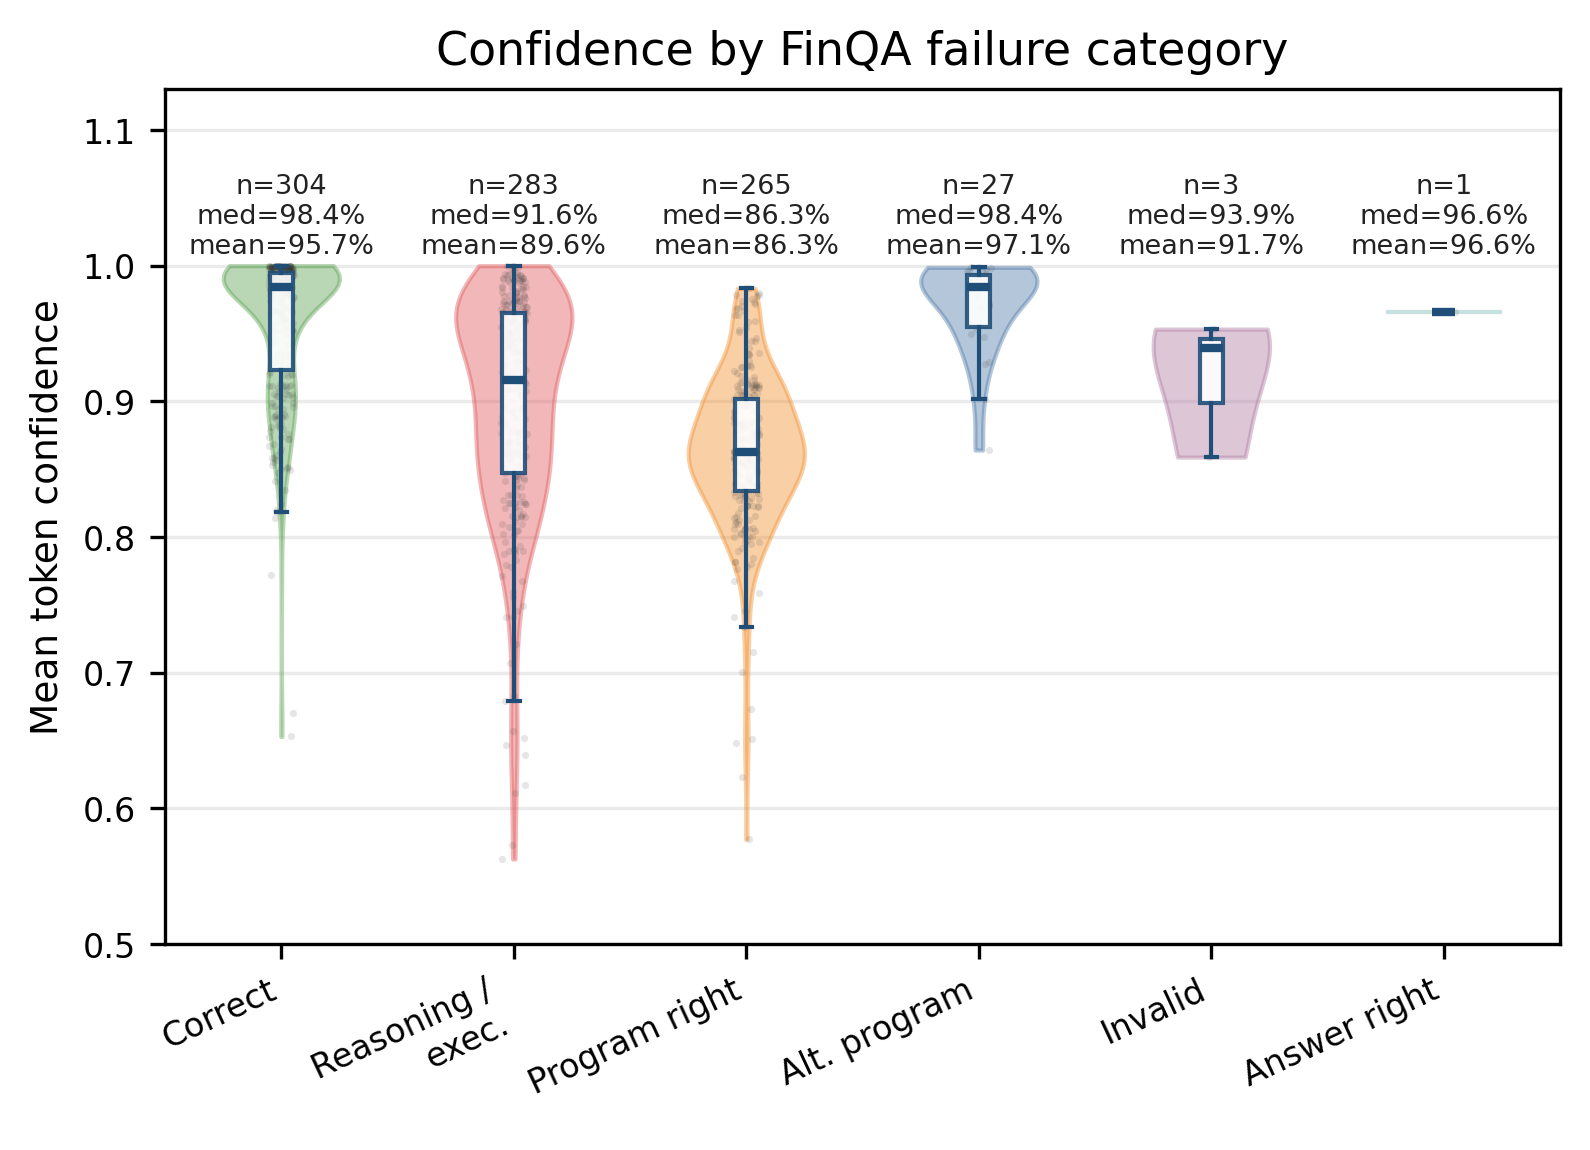
\includegraphics[width=0.92\textwidth]{figures/fig3_finqa_confidence_by_failure.png}
\caption{\label{fig:finqa_conf_violin} Confidence distributions by failure type (FinQA
validation). Each violin is overlaid with individual observations, a box summary, and
explicit $n$, median, and mean values. Correct and reasoning-error records share nearly the
same confidence regime --- the model is equally confident when it is right and when its
program mis-specifies the gold computation, which is why raw log-probability cannot rank
errors and why the agreement feature is required for abstention.}
\end{figure}

\begin{figure}[t]
\centering
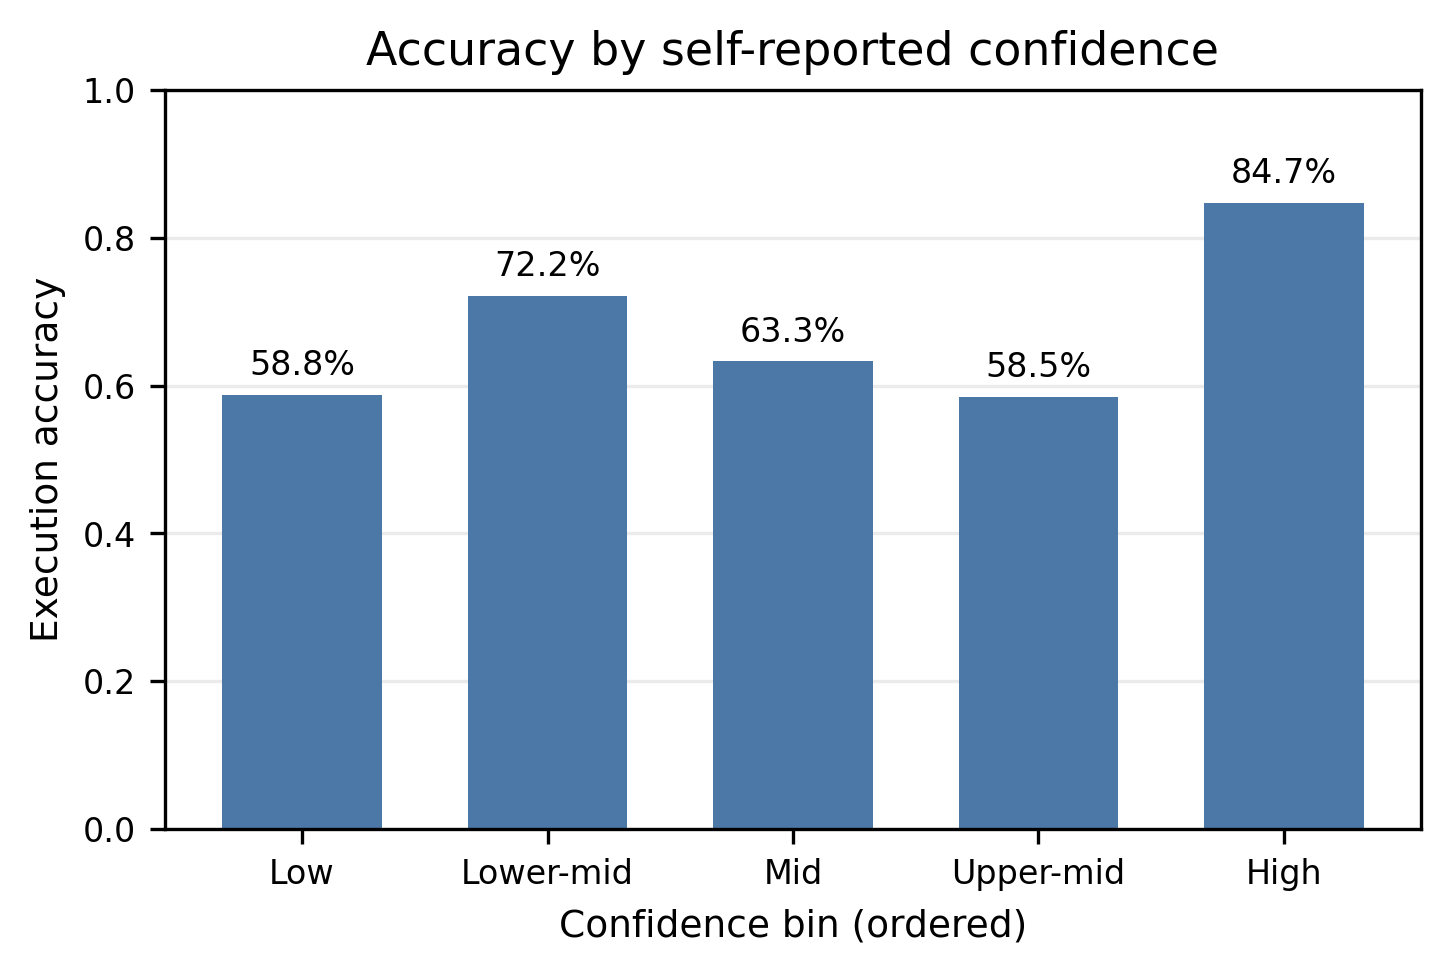
\includegraphics[width=0.92\textwidth]{figures/fig4_finqa_confidence_bins_accuracy.png}
\caption{\label{fig:finqa_bins} Execution accuracy by self-reported confidence bin
(FinQA validation, $n{=}883$). The 70--80\% bin is \emph{less} accurate than $\le$70\%
(2.3\% vs.\ 11.8\%), confirming the non-monotone raw-confidence ranking that motivates
the multi-feature Platt calibrator (Table~\ref{tab:calib}).}
\end{figure}

\begin{figure}[t]
\centering
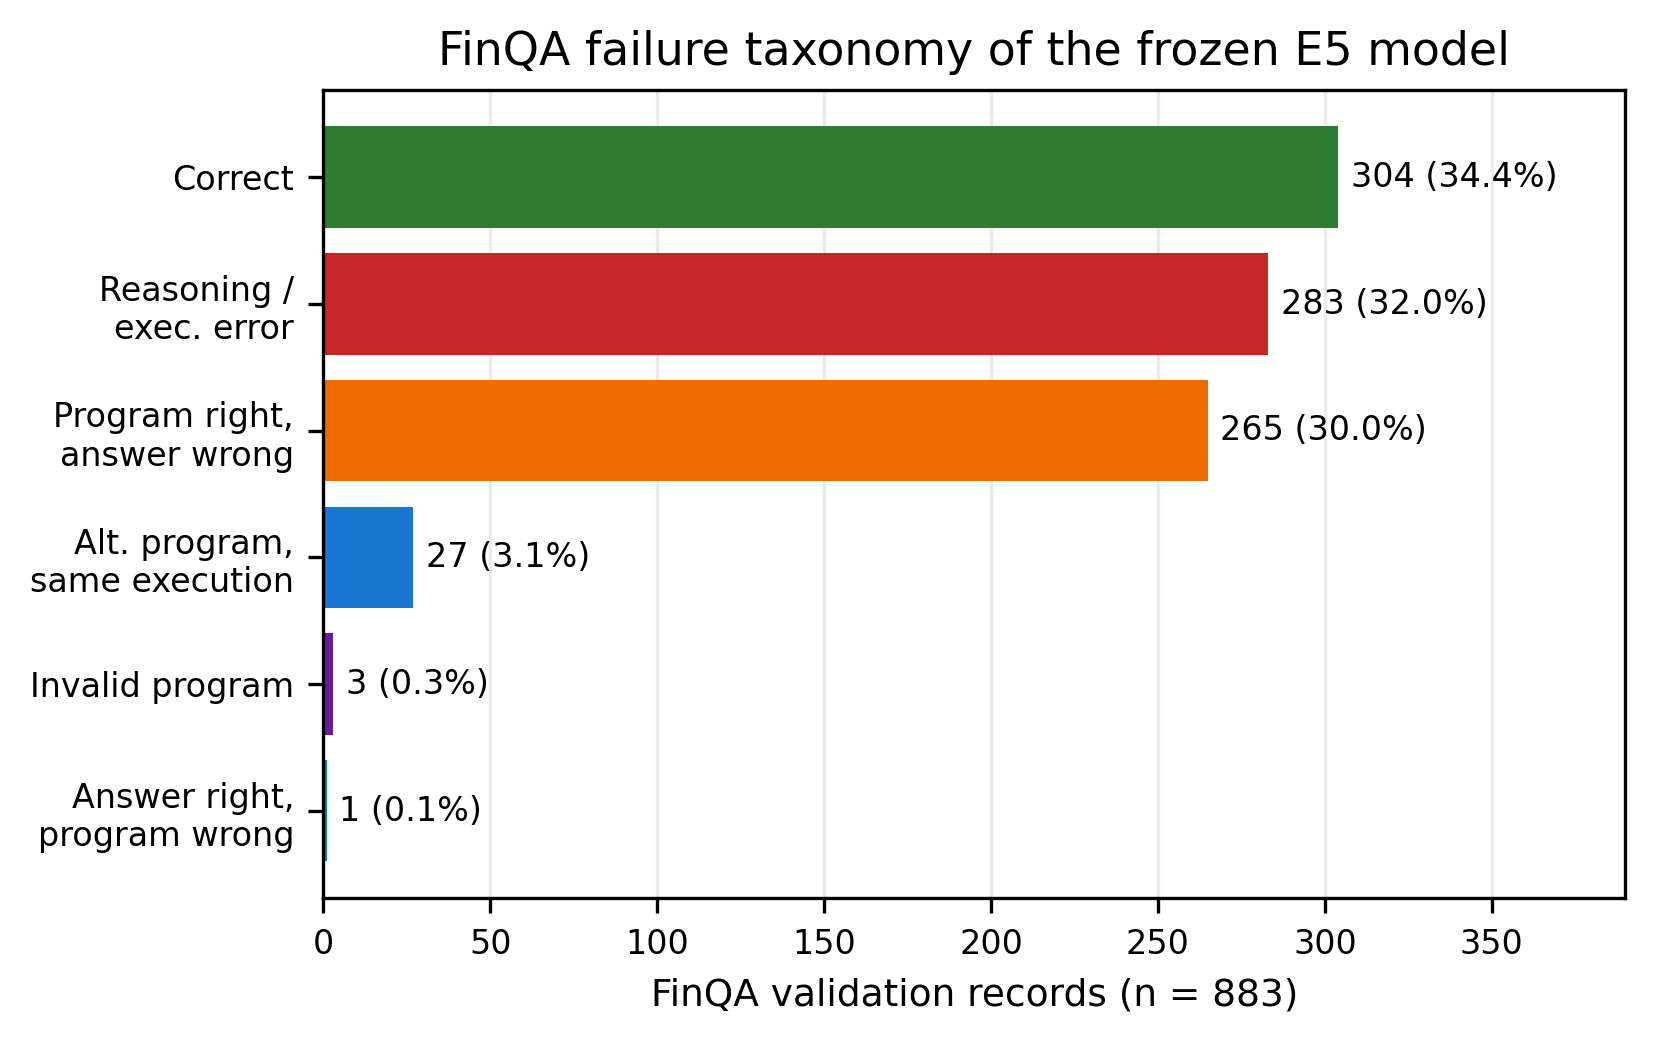
\includegraphics[width=0.8\textwidth]{figures/fig1_finqa_failure_taxonomy.png}
\caption{\label{fig:finqa_taxonomy} FinQA failure taxonomy (counts and share of all
validation records).}
\end{figure}

\paragraph{Rigor, error taxonomy, and depth (Table~\ref{tab:rigor}).}
The protected test was opened once against the frozen manifest. Per-record significance
testing formalises the C1 verdict; the remaining error is not parsing (0/1,147) and not
program validity (0 for EVG), but 34.4\% genuine arithmetic slips. The validation-side
failure distribution (Figures~\ref{fig:finqa_failure}--\ref{fig:finqa_taxonomy}) sharpens
this picture: the residual splits into near-miss answer errors (median relative error
1.7\%) and catastrophic reasoning misreads (median $\approx$99\%), and raw confidence is
nearly identical in the correct and failed classes --- the quantitative motivation for
the agreement-based calibrator. Greedy additionally
suffers a 31.0\% formatting channel --- the correct value is computed yet a different
string is printed --- which EVG's \texttt{exec\_verified} rule removes by construction.
Stratifying by the FinQA program-depth proxy, the frozen policy abstains least on 0-op
lookups (4.4\%) and most on 3--6-op programs (31.3\%), where it cuts error by 41.7\%:
abstention cost is spent precisely where reasoning is deepest. All numbers carry bootstrap
CIs in the annexed rigor report; the calibration threshold used here was frozen on
validation and never touched after the test opened.

\paragraph{Out-of-domain robustness.}
Table~\ref{tab:fomc}. Without any FOMC data in training, the frozen adapter raises macro-F1
0.21 $\rightarrow$ 0.30 and parse success 0.90 $\rightarrow$ 0.99, with the gain in the
rare classes (dovish F1 0.16 $\rightarrow$ 0.33; hawkish 0.05 $\rightarrow$ 0.26).

\paragraph{Cost.} EVG at $n=8$ runs at 4.8~s/question vs.\ 1.3~s greedy (3.7$\times$,
shared prefill), peak VRAM 3.1~GB / 6~GB.

\section{Discussion and limitations}
\textbf{What we did not claim.} EVG-CAS does not raise accuracy; reporting a tie, rather
than a $p$-value-won headline, is the point of the pre-registration. \textbf{Domain limits.}
On FiQA (117 validation / 234 test records, regression), the EVG features carry no signal
and the frozen policy correctly abstains to no effect --- a second reported negative result.
\textbf{General limits.} One backbone, one seed, one evaluation harness; between-seed
variance of the agreement signal is unmeasured; $n{=}8$ is pre-declared, not tuned; the
abstention gain costs 3.7$\times$ latency for zero accuracy gain. \textbf{Threats to
validity.} The protected-test protocol rests on the frozen manifest hash being unchanged
across access (it is); any leakage would invalidate C3's transfer claim. \textbf{Ethics.}
Abstention is a refusal signal, not a guarantee; a deployed system that \emph{answers} still
carries residual error (23.8\% at coverage 0.8). No financial advice is implied.

\section{Conclusion}
For a QLoRA-adapted 1.7B financial model, execution-verified generation ties greedy decoding
on accuracy but produces a steep, monotone agreement signal that the model's own confidence
cannot see. Calibrating that signal yields a pre-registered abstention threshold that
transfers to a once-opened protected test, cutting answered-error by 31\% at 80\% coverage.
The contribution to the financial-SLM conversation is that generation-level verification
does not make a small model \emph{right} more often --- it makes it \emph{know when it is wrong},
which is the property finance deployment needs most. Artifacts, frozen manifest and the full
experiment trail are public; \texttt{P4-E9} (FinTrust per-dimension evaluation) is the
declared next step.

\small
\begin{thebibliography}{99}
\bibitem{chen2021finqa} Z.~Chen \emph{et al.}, ``FinQA: A Dataset of Numerical Reasoning over Financial Data,'' EMNLP, 2021.
\bibitem{chen2022convfinqa} Z.~Chen \emph{et al.}, ``ConvFinQA: Exploring the Chain of Numerical Reasoning in Conversational Finance Question Answering,'' EMNLP, 2022.
\bibitem{zhu2021tatqa} F.~Zhu \emph{et al.}, ``TAT-QA: A Question Answering Benchmark on a Hybrid of Tabular and Textual Content in Finance,'' ACL, 2021.
\bibitem{phogat2024finetuning} K.~Singh~Phogat \emph{et al.}, ``Fine-tuning Smaller Language Models for Question Answering over Financial Documents,'' Findings of EMNLP, 2024.
\bibitem{yang2023fingpt} H.~Yang, X.-Y.~Liu, C.~D.~Wang, ``FinGPT: Open-Source Financial Large Language Models,'' J. Financial Data Science (arXiv:2306.06031), 2023.
\bibitem{yang2023investlm} Y.~Yang, Y.~Tang, K.~Y.~Tam, ``InvestLM: A Large Language Model for Investment using Financial Domain Instruction Tuning,'' arXiv:2309.13064, 2023.
\bibitem{wu2023bloomberg} S.~Wu \emph{et al.}, ``BloombergGPT: A Large Language Model for Finance,'' arXiv:2303.17564, 2023.
\bibitem{huang2020finbert} A.~Huang, H.~Wang, Y.~Yang, ``FinBERT: A Pretrained Language Model for Financial Communications,'' arXiv:2006.08097, 2020.
\bibitem{shi2025kronos} Y.~Shi \emph{et al.}, ``Kronos: A Foundation Model for the Language of Financial Markets,'' arXiv:2508.02739, 2025.
\bibitem{xie2024finben} Q.~Xie \emph{et al.}, ``FinBen: A Holistic Financial Benchmark for Large Language Models,'' NeurIPS D\&B, 2024.
\bibitem{hu2025fintrust} T.~Hu \emph{et al.}, ``FinTrust: A Comprehensive Benchmark of Trustworthiness Evaluation in Finance Domain,'' EMNLP, 2025.
\bibitem{subramanian2025slms} S.~Subramanian \emph{et al.}, ``Small Language Models (SLMs) Can Still Pack a Punch: A Survey,'' arXiv:2501.05465, 2025.
\bibitem{abdin2024phi3} M.~Abdin \emph{et al.}, ``Phi-3 Technical Report,'' arXiv:2404.14219, 2024.
\bibitem{zhang2024tinyllama} P.~Zhang \emph{et al.}, ``TinyLlama: An Open-Source Small Language Model,'' arXiv:2401.02385, 2024.
\bibitem{qwen2025qwen3} Qwen Team, ``Qwen3 Technical Report,'' arXiv:2505.09388, 2025.
\bibitem{hu2022lora} E.~Hu \emph{et al.}, ``LoRA: Low-Rank Adaptation of Large Language Models,'' ICLR, 2022.
\bibitem{dettmers2023qlora} T.~Dettmers \emph{et al.}, ``QLoRA: Efficient Finetuning of Quantized LLMs,'' NeurIPS, 2023.
\bibitem{wang2023selfconsistency} X.~Wang \emph{et al.}, ``Self-Consistency Improves Chain of Thought Reasoning in Language Models,'' ICLR, 2023.
\bibitem{lightman2024verify} H.~Lightman \emph{et al.}, ``Let's Verify Step by Step,'' ICLR, 2024.
\bibitem{wang2024mathshepherd} P.~Wang \emph{et al.}, ``Math-Shepherd: Verify and Reinforce LLMs Step-by-step without Human Annotations,'' ACL, 2024.
\bibitem{chen2019execution} X.~Chen, D.~Song, Y.~Tian, ``Execution-Guided Neural Program Synthesis,'' ICLR, 2019.
\bibitem{eliyaniv2010selective} R.~El-Yaniv, Y.~Wiener, ``On the Foundations of Noise-free Selective Classification,'' JMLR 11, 2010.
\bibitem{geifman2017selective} Y.~Geifman, R.~El-Yaniv, ``Selective Classification for Deep Neural Networks,'' NeurIPS, 2017.
\bibitem{geifman2019selectivenet} Y.~Geifman, R.~El-Yaniv, ``SelectiveNet: A Deep Neural Network with an Integrated Reject Option,'' ICML, 2019.
\bibitem{guo2017calibration} C.~Guo \emph{et al.}, ``On Calibration of Modern Neural Networks,'' ICML, 2017.
\bibitem{platt1999platt} J.~C.~Platt, ``Probabilistic Outputs for Support Vector Machines and Comparisons to Regularized Likelihood Methods,'' Advances in Large Margin Classifiers, 1999.
\bibitem{zadrozny2002isotonic} B.~Zadrozny, C.~Elkan, ``Transforming Classifier Scores into Accurate Multiclass Probability Estimates,'' KDD, 2002.
\bibitem{lin2022uncertainty} S.~Lin, J.~Hilton, O.~Evans, ``Teaching Models to Express Their Uncertainty in Words,'' TMLR, 2022.
\bibitem{fritzmorgenthal2022risk} S.~Fritz-Morgenthal, B.~Hein, J.~Papenbrock, ``Financial Risk Management and Explainable, Trustworthy, Responsible AI,'' SSRN 3873768, 2022.
\end{thebibliography}

\end{document}